% RQ4
\newpage
\section{Interpretability of tools}
\label{sec:interpretabilityoftools}
Finally, this section will cover research question 4: \textit{Do these data profiles provide more interpretability of error detection tools?};

Based on \autoref{sec:performanceprediction} and \autoref{sec:toolranking}, with a set of input features and output values in the two tasks, the regression models can be analyzed to "explain" the inner workings of tools. Using feature importance identification methods depending on the specific regressor or general importance methods, the "weight" of a certain feature of the data profile can be translated to the performance of a certain tool with a specific configuration. The importance of features for each strategy can than be analyzed, to see if they correspond with the underlying techniques in these methods. If there are matches and mismatches, try to find why the misalignment occurs and see if improvements can be suggested for the error detection tools. A visual representation of making the error detection models interpretable, is shown in \autoref{fig:method_interpret}.

\begin{figure}[h]
    \centering
    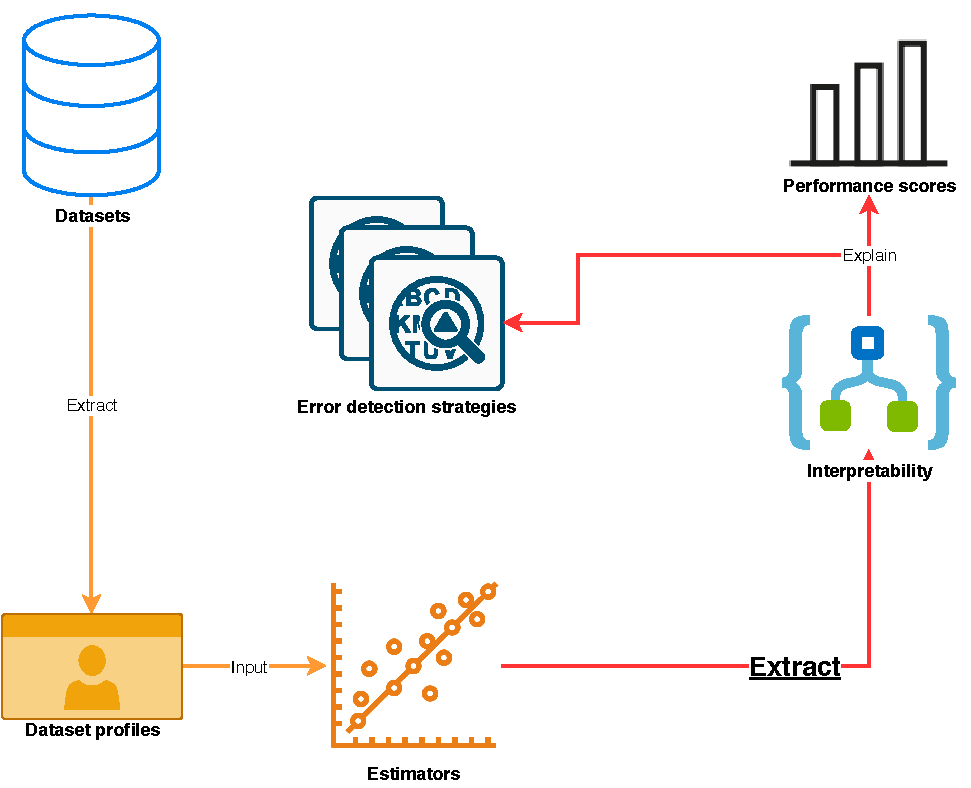
\includegraphics[width=0.9\textwidth]{thesis/Figures/Method/PerformanceEstimation-Interpretability.pdf}
    \caption{Adding interpretability into the flow of error detection}
    \label{fig:method_interpret}
\end{figure}

\subsection{Feature selection}
\label{subsec:featureselection}
Besides the learnable feature selection that will be used in the performance estimate pipeline of \autoref{sec:performanceprediction}, feature selection can also be done at the end of the estimation loop. For this part, permutation importance will be used to determine which features contribute to the estimation results. All features that actually seem to have positive impact on the model, will be kept for the dataset profile with less features. With this reduced number of features, the performance prediction of \autoref{sec:performanceprediction} will be repeated, to see if there is an improvement in estimation.

\subsection{Feature importance}
% According to the regression models
% Used as a proxy, something that is easy and quick to measure
Finding which data profile features are important for the estimator model to estimate its performance, give insights to how a certain error detection strategy behaves.

To answer whether the dataset profile features could provide more insight on when and how the selected error detection tools perform correctly, the direct F1-score, recall and precision estimators from \autoref{sec:performanceprediction} will be analyzed using SHAP values. For each tool, the best performing configuration (highest mean F1-score) will be analyzed. First, the features with the highest impact on the estimator output will be inspected. Then, the correlation between the most impacting features and the SHAP contribution of that feature will be calculated to find if higher or lower feature values have positive or negative impact on the model outputs. 

\subsection{Evaluation}
To evaluate Research Question 4: \textit{Do these data profiles provide more interpretability of error detection tools?};
there will be an analysis of both the feature selection and feature importance part of this section. 

The feature selection results produced from repeating the experiments from \autoref{sec:performanceprediction} will be compared on the mean squared error and mean absolute error to check for improvements. These comparisons will be done for performance metrics (precision, recall and direct F1 estimation), as well as for the combined F1 estimation.
If there is a clear improvement in mean squared error and mean absolute error, it will show that automated interpretability can be beneficial for the estimator models.

The main focus of evaluation will lie on the produced feature importance, explained by the second experiment in the section above. Finding the most impactful features and their correlation with the performance scores could be useful for interpretability if for every tool:
\begin{itemize}
    \item The top features have a strong impact on the estimator model output
    \item The correlations are translatable to theories or logic about the features impact on the model output
\end{itemize}

If both requirements can be met, the dataset profiles will add more interpretability of when, how and if the error detection tools will perform properly.